\chapter{แนวคิด ทฤษฎีและงานวิจัยที่เกี่ยวข้อง}
\label{chapter:related-theory}

\section{ระบบให้การแนะนำ (Recommendation System)}
ระบบให้การแนะนำ \cite[baptiste]{baptiste} เป็นระบบสนับสนุนการตัดใจที่จะให้การแนะนำสินค้าหรือบริหารที่มีความเหมาะสมกับรูปแบบและพฤติกรรมของลูกค้าหรือยูสเซอร์แต่ละคน โดยอาศัยข้อมูลของยูสเซอร์งานร่วมกับข้อมูลประกอบภายนอกมาใช้ในการวิเคราะห์คัดกรอง ให้ได้สิ่งที่มีความหมายที่เหมาะสมกับยูสเซอร์งาน โดยมีเทคนิคแบ่งย่อยได้เป็นสองชนิดหลัก ๆ คือ การกรองแบบอิงเนื้อหา (Content Based Filtering) การกรองแบบร่วม (Collaborative Filtering) และการกรองแบบผสม (Hybrid Recognition) \cite{robin}

\begin{figure}[!h]
  \centering
  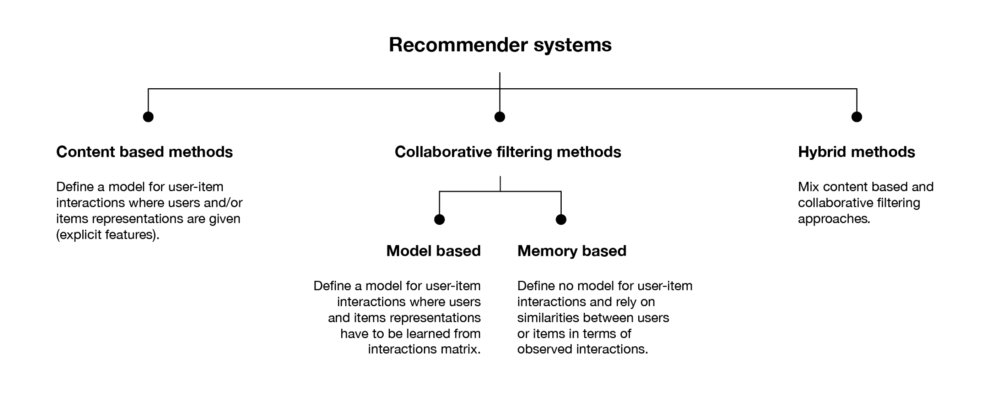
\includegraphics[width=1\textwidth]{colla_content_overall.png}  
  \caption{\cite[baptiste]{baptiste}อัลกอริทึมระบบผู้แนะนำประเภทต่างๆ}
  \label{Fig:cell-and-block}
\end{figure}

\subsection{การกรองแบบร่วมกัน (Collaborative Filtering)}
\begin{figure}[!h]
  \centering
  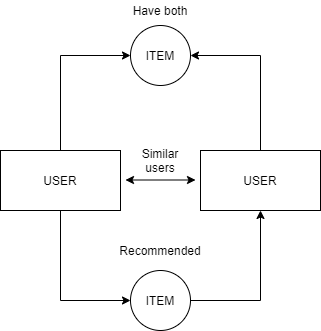
\includegraphics[width=0.4\textwidth]{CF.png}  
  \caption{ภาพรวมการกรองแบบร่วมกัน}
  \label{Fig:cell-and-block}
\end{figure}
การกรองแบบร่วม เป็นเทคนิคและนำโดยใช้ข้อมูลการโต้ตอบในอดีตที่ถูกบันทึกไว้ระหว่างยูสเซอร์และรายการเพื่อสร้างคำแนะนำใหม่ ๆ โดยข้อมูลเหล่านี้จะถูกเก็บไว้ในรูปแบบเมทริกซ์ที่เรียกว่า "user-item interactions matrix"
\newline
\begin{figure}[!h]
  \centering
  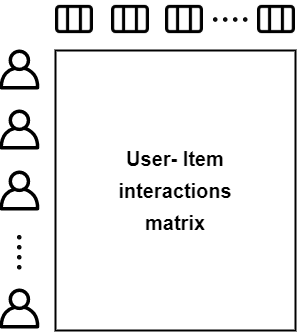
\includegraphics[width=0.3\textwidth]{colla_01.png}  
  \caption{เมทริกซ์การโต้ตอบยูสเซอร์ไอเทม}
  \label{Fig:cell-and-block}
\end{figure}

แนวคิดหลักที่เป็นกฎของการกรองแบบร่วมกันคือข้อมูลการโต้ตอบในอดีตในประมาณที่มากเพียงพอจะสามารถตรวจหาความคล้ายคลึงกันของยูสเซอร์กับไอเทมหรือยูสเซอร์กับยูสเซอร์ได้ 
คลาสของอัลกอริธึมการกรองแบบร่วมกันแบ่งออกเป็นสองประเภทย่อยที่โดยทั่วไปเรียกว่า อิงจากหน่วยความจำ (memory based) และ อิงจากโมเดล (model based) ในวิธีนี้การทำงานจะไม่มีการสันนิษฐานแบบจำลองแฝงแต่อัลกอริทึมจะทำงานโดยตรงกับข้อมูลการตอบโต้ยูสเซอร์และไอเทม ตัวอย่างเช่น ยูสเซอร์จะแสดงผลลัพธ์ของข้อมูลไอเทมเพื่อนบ้านที่ใกล้เคียงที่สุดเพื่อใช้ในการแนะนำ วิธีนี้จะมีความอคติต่ำในทางทฤษฎีแต่มีความแปรปรวนสูง 
และการอิงจากโมเดล วิธีนี้ถือว่าเป็นรูปแบบปฎิสัมพันธ์แฝง โมเดลนี้จะได้รับการฝึกให้สร้างค่าการตอบโต้ยูสเซอร์ไอเทมใหม่จากการแสดงยูสเซอร์และไอเทมของตัวเอง จากนั้นคำแนะนำใหม่สามารถทำได้โดยใช้โมเดลนี้ การทำนายจะมีความหมายทางคณิตศาสตร์ที่ยากต่อการตีความโดยมนุษย์ ดังนั้นวิธีการนี้ถือว่าเป็นวิธีที่มีความอคติสูงแต่มีความแปรปรวนต่ำ
\newline
\begin{figure}[!h]
  \centering
  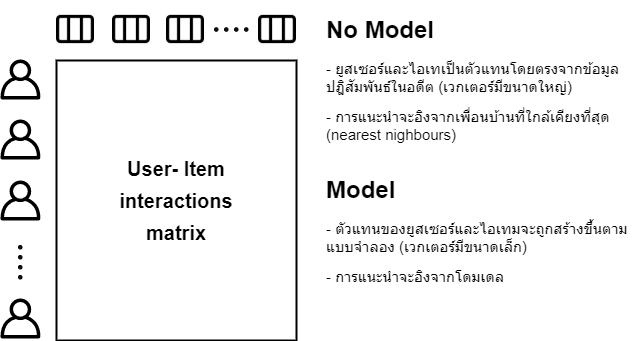
\includegraphics[width=0.8\textwidth]{colla_02.png}  
  \caption{ภาพรวมของกระบวนทัศน์วิธีการกรองร่วมกัน}
  \label{Fig:cell-and-block}
\end{figure}
\pagebreak

ข้อได้เปรียบหลักของการกรองแบบร่วมกันคือไม่ต้องการข้อมูลเกี่ยวกับยูสเซอร์หรือรายการเป็นตัวตั้งต้น ดังนั้นจึงสามารถใช้ได้ในหลายสถานการณ์ ยิ่งไปกว่านั้นยิ่งข้อมูลการโต้ตอบมีมากขึ้นเท่าใด คำแนะนำใหม่ก็จะยิ่งถูกต้องมากขึ้นเท่านั้น
แต่ถึงอย่างนั้นเนื่องจากไม่ต้องการข้อมูลในการตั้งต้นการพิจารณ์ข้อมูลเพื่อแนะนำจึงเกิดปัญหา นั่นคือ "cold start problem" ในทางปฎิบัติจึงเป็นไปไม่ได้ที่จะแนะนำสิ่งใดให้กับยูสเซอร์ใหม่หรือแนะนำรายการใหม่ให้กับยูสเซอร์ ยูสเซอร์และรายการที่มีข้อมูลการตอบโต้ที่น้อยเกินไปจะทำให้การแนะนำคลาดเคลื่อนเป็นอย่างมาก, ปัญหานี้สามารถแก้ไขได้หลายวิธีอย่างเช่น การแนะนำไอเทมแบบสุ่มให้กับยูสเซอร์ใหม่หรือแนะนำไอเทมใหม่กับยูสเซอร์แบบสุ่ม หรือการแนะนำไอเทมยอดนิยมให้กับยูสเซอร์ใหม่หรือไอเทมใหม่ให้กับยูสเซอร์ส่วนใหญ่ หรือการแนะนำชุดรายการให้กับยูสเซอร์ใหม่หรือรายการใหม่ไปยังกลุ่มยูสเซอร์ที่หลากหลายเป็นต้น

\pagebreak
\subsubsection{Memory Based}
\paragraph{User-user}
ในการแนะนำให้กับยูสเซอร์ วิธี user-user จะพยามระบุผู้ใช้ที่มีข้อมูลโปรไฟล์การโต้ตอบที่คล้ายคลึงกันมากที่สุด (เพื่อนบ้านที่ใกล้ที่สุด) เพื่อแนะนำรายการที่ได้รับความนิยมมากที่สุดให้บรรดาเพื่อนบ้านเหล่านี้ (หมายถึงยูสเซอร์ใหม่) วิธีนี้เรียกว่า "ผู้ใช้เป็นศูนย์กลาง" (user-centred)
สมมติว่าเราต้องการให้คำแนะนำสำหรับยูสเซอร์ใหม่ ขั้นแรกทุกคนจะถูกแทนที่ด้วยเวกเตอร์ของการโต้ตอบกับรายการ หลังจากนั้นเราสามารถคำนวนความคล้ายคลึงกันระหว่างยูสเซอร์ที่เราสนใจกับยูสเซอร์อื่น ๆ ทุกคน การวัดความคล้ายคลึงกันคือการที่ยูสเซอร์สองคนมีปฎิสัมพันธ์คลายคลึงกันในรายการเดียวกันนั่นหมายความว่าควรได้รับการพิจารณาว่าอยู่ใกล้กัน เมื่อคำนวนความคล้ายคลึงกับยูสเซอร์ทุกคนแล้ว เราสามารถเก็บ k-nearest-nightbour ไว้ให้กับยูสเซอร์ของเราจากนั้นแนะนำรายการที่ได้รับความนิยมมากที่สุดในบรรดารายการเหล่านี้
\newline
\begin{figure}[!h]
  \centering
  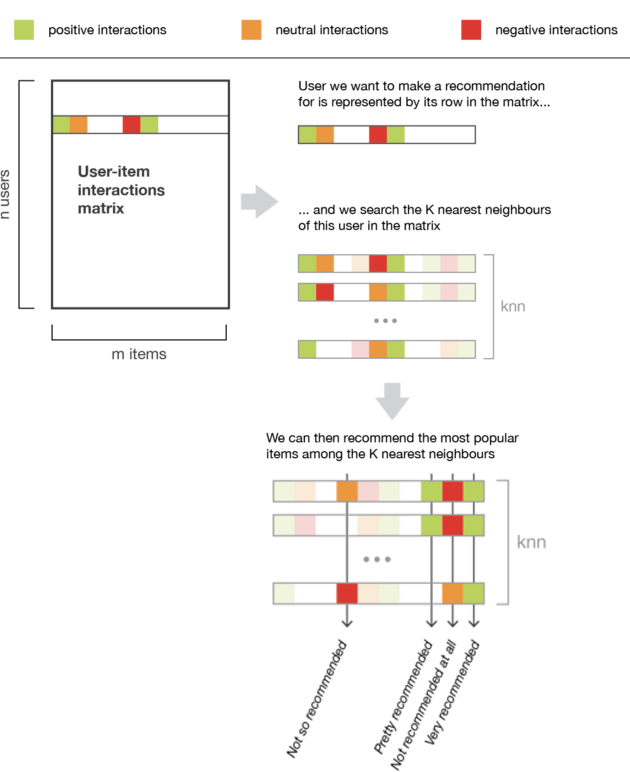
\includegraphics[width=0.8\textwidth]{content_user_user.png}  
  \caption{\cite[baptiste]{baptiste} วิธีการแบบ user-user}
  \label{Fig:cell-and-block}
\end{figure}
\paragraph{Item-item}
การให้คะแนะนำใหม่แก่ยูสเซอร์แนวคิดของวิธี item-item คือการหารายการที่สอดคล้องกับรายการที่ยูสเซอร์มีรายการตอบโต้เป็นบวก (position) สองรายการซึ่งจะถือว่าคล้ายกันหากผู้ใช้ส่วนใหญ่ที่มีปฎิสัมพันธ์กับทั้งคู่ทำในลักษณะเดียวกัน วิธีนี้เรียกว่า "item-centred"
\newline
\begin{figure}[!h]
  \centering
  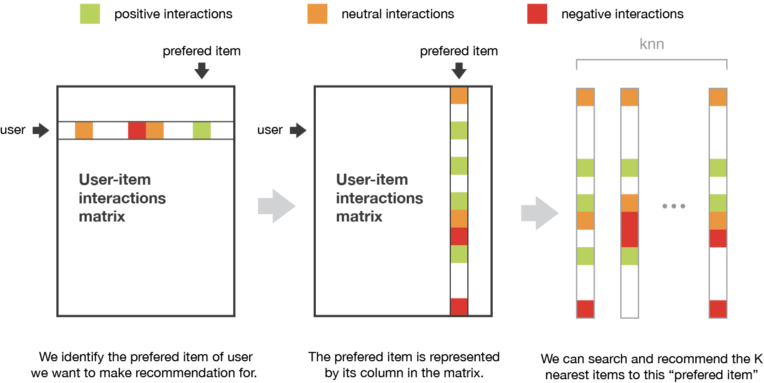
\includegraphics[width=1\textwidth]{content_item_item.png}  
  \caption{\cite[baptiste]{baptiste} วิธีการแบบ item-item}
  \label{Fig:cell-and-block}
\end{figure}
\subsubsection{Model Based}
การกรองแบบร่วมกันโดยใช้โมเดล อาศัยข้อมูลการโต้ตอบยูสเซอร์ไอเทม และใช้โมเดลในการอธิบายข้อมูลการโต้ตอบเหล่านี้ ตัวอย่างเช่น อัลกอริธึมการแยกตัวประกอบเมทริกซ์ (matrix factorisation) โดยสลายเมทริกซ์การโต้ตอบยูสเซอร์ไอเทมที่มีขนาดใหญ่และกระจายให้ให้เป็นตารางเมทริกซ์ที่มีขนาดเล็กและหนาแน่นจำนวนสองเมทริกซ์
% \paragraph{Matrix factorisation}
% อัลกอริธึมการแยกตัวประกอบเมทริกซ์ (matrix factorization) ทำงานโดยการแยกเมทริกซ์ข้อมูลการโต้ตอบยูสเซอร์ไอเทมออกเป็นผลคูณของเมทริกซ์สองมิติที่มีมิติต่ำกว่าสองตัวที่สามารถคูณกันแล้วได้เมทริกซ์เป้าหมาย
% ตัวอย่าง, มีเมทริกซ์การให้คะแนนภาพยนต์ของยูสเซอร์ เราสามารถสันนิษฐานได้ว่า:
% \begin{itemize}
  %   \item มีคุณสมบัติบางอย่างที่อธิบาย (และแยกส่วน) ภาพยนต์ได้ดีอยู่
  %   \item คุณสมบัติเหล่านี้สามารถใช้เพื่ออธิบายยูสเซอร์ได้
  % \end{itemize}
  % \begin{figure}[!h]
    %   \centering
    %   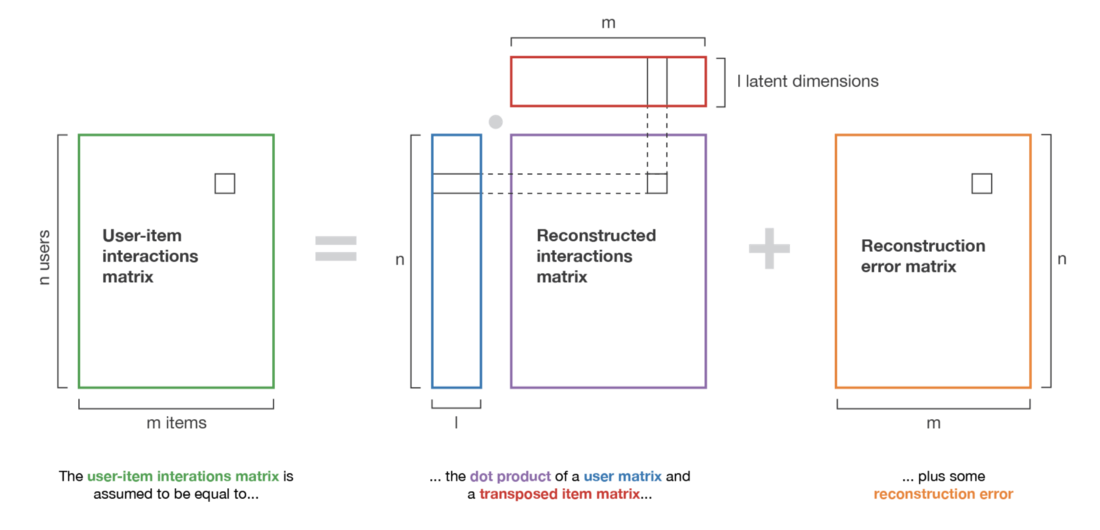
\includegraphics[width=1\textwidth]{matrix_factorization.png}  
    %   \caption{\cite[baptiste]{baptiste} matrix factorization}
    %   \label{Fig:cell-and-block}
    % \end{figure}
\pagebreak
    

\subsection{การกรองแบบอิงเนื้อหา (Content Based Filtering)}
\begin{figure}[!h]
  \centering
  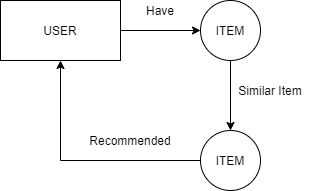
\includegraphics[width=0.4\textwidth]{CB.png}  
  \caption{ภาพรวมการกรองโดยอิงจากเนื้อหา}
  \label{Fig:cell-and-block}
\end{figure}
การกรองโดยอิงจากเนื้อหาต่างจากการกรองแแบบร่วมกันที่อาศัยข้อมูลการตอบโต้ยูสเซอร์และไอเทม การกรองโดยอิงจากเนื้อหาใช้ข้อมูลเพิ่มเติมเกี่ยวกับยูสเซอร์ และ/หรือ ไอเทม ยกตัวอย่างเช่นระบบแนะนำภาพยนต์ 
ข้อมูลเพิ่มเติมนี้อาจจะเป็น เพศ, อายุ, งาน หรือข้อมูลส่วนตัวอื่นๆ ของยูสเซอร์ เพราะฉะนั้นแนวคิดนี้คือการพยามสร้างแบบจำลองตามคุณลักษณะเพื่อพยามอธิบายยูสเซอร์และไอเทม ตัวอย่างเช่น เมื่อพิจารณ์ภาพยนต์ เราจะพยามจำลองความจริงที่ว่าผู้หญิงมักจะให้คะแนนภาพยนต์บางเรื่องตามที่เพศหญิงชอบ และผู้ใช้จะให้คะแนนภาพยนต์บางเรื่องตามที่เพศตัวเองชอบ เป็นต้น หากทำการพิจารณ์จากตัวอย่างข้างต้นเราเพียงแค่ดูโปรไฟล์เพศเราก็สามารถแนะนำภาพยนต์ที่เพศนั้นๆ ชอบได้
\newline
\begin{figure}[!h]
  \centering
  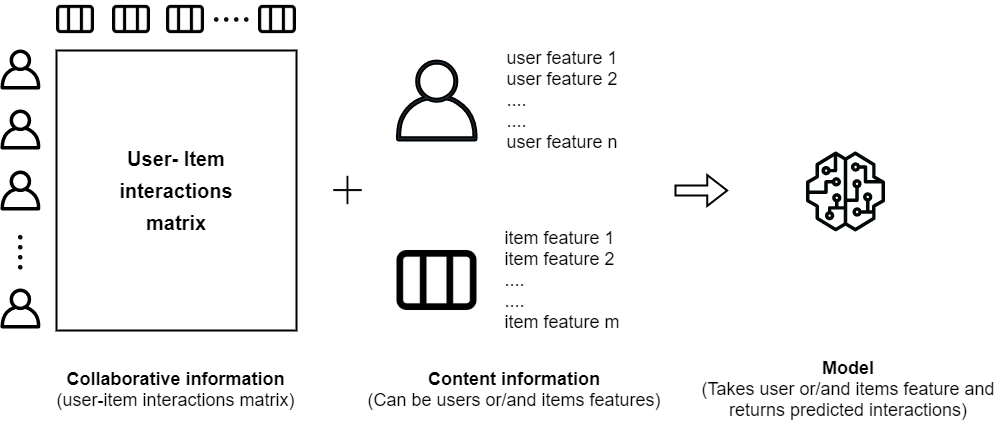
\includegraphics[width=1\textwidth]{content_01.png}  
  \caption{ภาพรวมของกระบวนทัศน์วิธีการกรองโดยอิงจากเนื้อหา}
  \label{Fig:cell-and-block}
\end{figure}
วิธีการอิงจากเนื้อหานั้นไม่จะประสบปัญหา "cold start problem" น้อยกว่าวิธีการอิงแบบร่วมกัน ยูสเซอร์ใหม่หรือไอเทมใหม่สามารถอธิบายได้ตามลักษณะ (เนื้อหา) ของตัวมันเอง และคำแนะนำที่เกี่ยวข้องสามารถทำได้สำหรับเอนทิตีใหม่เหล่านี้ เฉพาะยูสเซอร์ใหม่หรือผู้ใช้ใหม่ที่มีคุณสมบัติที่ไม่เคยเจอมาก่อนเท่านั้นที่ได้รับผลกระทบจากข้อเสียนี้ แต่เมื่อมีข้อมูลมากเพียงพอปัญหานี้จะหมดไป
\pagebreak

\subsection{ระบบให้การแนะนำแบบผสม (Hybrid Recommendation)}
ระบบการแนะนำแบบผสม เป็นการรวมการทำงานของระบบแนะนำที่ใช้เทคนิคการกรองแบบร่วม (Collaborative Filtering) และระบบแนะนำจากการกรองโดยอิงจากเนื้อหา (Content Based Filtering) เข้าด้วยกันเพื่อประสิทธิภาพที่ดียิ่งขึ้น และแก้ไขข้อด้อยของแต่ละเทคนิคเช่น การกรองแบบร่วมที่มีปัญหาใหญ่คือ Cold Start \cite{farshad} ที่ต้องการข้อมูลตั้งต้นเป็นจำนวนหนึ่งเพื่อจะได้แนะนำได้อย่างถูกต้อง ตรงจุดการกรองโดยอิงจากเนื้อหาสามารถแก้ไขจุดด้อยตรงนี้ได้เนื่องจากการกรองโดยอิงจากเนื้อหานั้น แค่จากโปรไฟล์ของเรากับไอเทมเป็นเเคสต่อเคสเท่านั้น
\newline
\begin{figure}[!h]
  \centering
  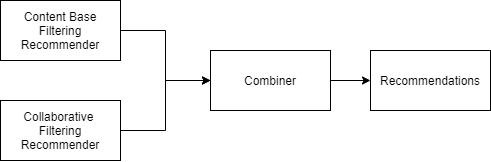
\includegraphics[width=0.8 \textwidth]{hybrid.png}  
  \caption{ขั้นตอนทำงาน การกรองแบบอิงเนื้อหา}
  \label{Fig:cell-and-block}
\end{figure}


\section{Apache Airflow}
Apache airflow \cite{airflow} เป็นแพลตฟอร์มการจัดการเวิร์กโฟลว์แบบโอเพนซอร์สามารถเขียนโปรแกรมเพื่อกำหนดเวลาขั้นตอนการทำงานและตรวจสอบผ่านอินเทอร์เฟชผู้ใช้ได้
Airflow เขียนด้วยภาษา python และเวิร์กโฟลว์ถูกสร้างผ่านสคริปต์ python โดยได้รับการออกแบบภายใต้หลักการ "configuration as code" แม้ว่าแพลตฟอร์มอื่น ๆ ที่ใช้หลักการนี้จะอยู่ภายใต้มารกอัปเช่น XML แต่การใช้ python ช่วยให้นักพัฒนานำเข้าไลบรารีและคลาสเพื่อช่วยในการสร้างเวิร์กโฟลว์ได้ง่ายและมีประสิทธิภาพมากยิ่งขึ้นกว่าการตั้งค่าโดด ๆ แบบ XML

Airflow ใช้กราฟ acyclic กำกับ (DAG) เพื่อจัดการระเบียบเวิร์ฟเฟลว์งาน และการอ้างอิงถูกกำหนดไว้ใน python จากนั้น airflow จะจัดการตั้งเวลาและดำเนินการ DAG ตามเวลาที่กำหนด (เช่น รายชั่วโมงรายวัน) หรือตามทริกเกอร์เหตุการภายนอก


\section{Docker}
Docker \cite{docker} เป็นเอ็นจิ้นที่มีการทำงานในลักษระจำลองสภาพวแดล้อมขึ้นมาบนเครื่องเซิรฟ์เวอร์เพื่อใช้ในการรันเซอร์วิสที่ต้องการ มีการทำงานคล้ายคลึงกับเครื่องเสมือน (virtual machine) เช่น MVWare, VirtualBox, XEN, KVM แต่ข้อแตกต่างที่ชัดเจนคือ เครื่องเสมือนที่กล่าวมาจำเป็นต้องจำลองทั้งระบบปฎิบัติการ (OS) เพื่อใช้งานและหากต้องการใช้บริการใด ๆ จำเป็นต้องติดตั้งเพิ่มบนระบบปฎิบัติการนั้น แต่สำหรับ docker แล้วจะใช้สิ่งที่เรียกว่าคอนเทนเนอร์ ในการจำลองสภาพแวดล้อมขึ้นมา เพื่อใช้งานสำหรับ 1 บริการ ที่ต้องการใช้งานเท่านั้น โดยไม่ต้องมีส่วนระบบปฎิบัติการเข้าไปเกี่ยวข้องด้วยเหมือนเครื่องเสมือนอื่น ๆ
\newline
\begin{figure}[!h]
  \centering
  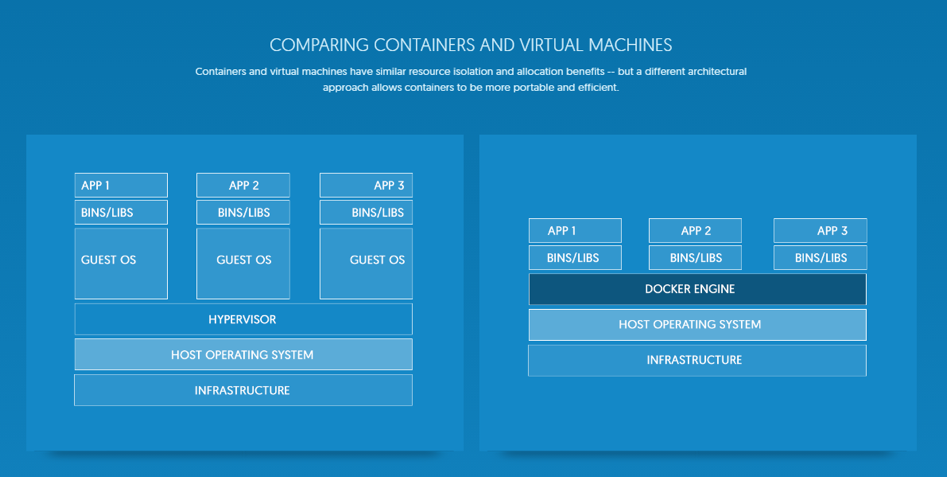
\includegraphics[width=1 \textwidth]{docker.png}  
  \caption{comparing container and virtual machines}
  \label{Fig:cell-and-block}
\end{figure}
โดย docker นั้นเป็นที่รู้จักกันอย่างแพร่หลายในช่วง 1-2 ปีที่ผ่านมานี้ เนื่องจากสามารถใช้งานได้อย่างสะดวกและตอบสนองความต้องการของผู้พัฒนาโปรแกรมหรือผู้ดูแลระบบ
\paragraph*{Docker image}
เป็นตัวต้นแบบของคอนเทนเนอร์ซึ่งภายในจะประกอบด้วยแอพพลิเคชั่นต่าง ๆ ที่มีการติดตั้งไว้เพื่อนใช้งานสำหรับบริการนั้น ๆ รวมทั้งมีการตั้งค่าต่าง ๆ ไว้อย่างเรียบร้อย จากนั้นจึงนำมาสร้างเป็นอิมเมจบนรีจิสทรีเพื่อนำมาใช้งานทั้งนี้ผู้ใช้งานสามารถสร้าง docker image ของตัวเองได้อีกด้วย
\paragraph*{Docker container}
เป็นกล่องเหสมือนซึ่งนำ docker image มาติดตั้งเพื่อให้สามารถใช้งานบริการที่ต้องการได้จากอิมเมจนั้น ๆ โดยในคอนเทนเนอร์แต่ละตัวจะมีการใช้งาน RAM, CPU ไฟล์ตั้งค่าต่าง ๆ เป็นของแต่ละคอนเทนเนอร์เอง


\section{การสกัดข้อมูล (Data Scraping)}
การสกัดข้อมูล \cite{choochart} เป็นเทคนิคในการเข้าถึงข้อมูลจากเว็บไซต์เพื่อที่หาและสกัดข้อมูลที่ต้องการ ในการสกัดข้อมูลจากข้อความที่ดึงมาจากเว็บไซต์สามารถใช้ไลบรารี่ beautifulsoup ของภาษา python เพื่อช่วยในการสกัดข้อมูลให้มีความง่ายขึ้นได้ กรณีที่เว็บไซต์ที่ทำงานโดยการเรนเดอร์หน้าเพจทั้งหน้าแล้วส่งมาให้ยูสเซอร์ (client) ราสามารถดึงข้อมูลของทั้งหน้ามาใช้ได้โดยตรงและสกัดข้อมูลจากที่กล่าวมาข้างต้น แต่บางเว็บไซต์ที่มีการทำงานแบบฝั่งไคลเอนต์ มีการแสดงผลข้อมูลเป็นแบบ Asynchronous ซึ่งทำให้ข้อมูลปรากฎขึ้นไม่พร้อมกัน โดยจะขึ้นอยู่กับการกระทำของยูสเซอร์เช่น คลิ๊กเปิด เลื่อนลงเพื่อโหลดฟีด จะไม่สามารถดึงข้อมูลทั้งหน้าได้จำเป็นต้องจำเป็นต้องแก้ปัญหาโดยทำการจำลองบราวเซอร์เพื่อจำลองการกระทำของยูสเซอร์ขึ้นมา
\subsection{Puppeteer}
Puppeteer เป็นไลบรารี่ Node ซึ่งมีอีพีไอระดับสูงเพื่อควบคุม Chrome หรือ Chromium ผ่านหน้าพัฒนา โดย puppeteer จะทำการรันเป็นเบราว์เซอร์ล่องหน (headless browser) หรือคือไม่มีอินเทอร์เฟซผู้ใช้งานแบบกราฟิกโดยเบราว์เซอร์ล่องหนสามารถควบคุมหน้าเว็บได้โดยอัติโนมัติในสภาพแวดล้อมที่คล้ายกับเว็บเบราว์เซอร์ แต่จำเดินการผ่านอินเทอร์เฟซบรรทัดคำสั่งหรือใช้การสื่อสารผ่านเครือข่าย มีประโยชน์เป็นอย่างมากสำหรับการทดสอบหน้าเว็บเนื่องจากสามารถแสดงผลและทำความเข้าใจ HTML ได้อีกทั้งยังสามารถประยุกต์ใช้เบราว์เซอร์ล่องหนในการสกัดข้อมูลจากเว็บไซต์ที่ต้องการผ่านการจำลองเสมือนเพื่อเข้าถึงข้อมูลที่ต้องการ 


\section{การประมวลผลภาษาธรรมชาติ (Natural Language Processing)}
การประมวลผลภาษาธรรมชาติ (NLP) \cite{diego} เป็นแขนงหนึ่งของสาขาปัญญาประดิษฐ์ (Artificial Intelligence) ที่ทำให้เครื่องจักรมีความสามารถในการอ่านทำความเข้าใจและเข้าใจความหมายของภาษามนุษย์ได้ กล่าวคือ NLP แสดงถึงการจัดการภาษามนุษย์โดยอัตโนมัติเช่นการพูด ข้อความ หรือแม้กระทั่งแนวคิดที่สนใจ โดยได้มีการนำไปประยุกต์ใช้ในแขนงมากมายเช่น ช่วยในการทำความเข้าใจและคาดการณ์กลุ่มของยูสเซอร์จากโปรไฟล์ของยูสเซอร์เหล่านั้น เป็นต้น

\subsection{Word Embedding}
Word Embedding \cite{lukkiddd} คือการจับบริบทของคำในเอกสารที่มีความคล้ายคลึงกับคำอื่น ๆ และแปลงคำให้เป็นตัวเลขในรูปแบบเว็กเตอร์ โดยถือเป็นหนึ่งในวิธีการสร้างฟีเจอร์จากคำวิธีหนึ่ง โดยทำการลดขนาดเว็กเตอร์ลงด้วย เช่น ทำการ word embedding กับคำว่า "I, liked, the, hotel" เราจะได้เวกเตอร์ออกมาคือ I[0.3, 0.2, 0.8, 0.1], liked[0.4, 1.2, 0.1, 0.9], the[1.3, -2.1, 0, 1.2], hotel[0.5, 1.4, 0.3, -0.4] เป็นต้น

\subsubsection{Word2Vec}
Word2Vec \cite{lukkiddd} Pre-trained weight model หรือแบบจำลองน้ำหนักที่ผ่านการเทรนมาล่วงหน้าแล้ว word2vec มีสองแบบที่สามารถใช้เพื่อทำ word embeddings คือ CBOW และ Skip-gram
\begin{enumerate}
  \item \textbf{Bag-of-Words Models (CBOW)} โดมเดลนี้จะทำนายคำถัดไปโดยอ้างอิงจาก n คำก่อนหน้าและ n คำต่อท้ายคำถัดไป ตัวอย่างเช่นประโยคต่อไปนี้ 
  
  \centerline{\emph{Lorem ipsum dolor sit amet}}
  
  CBOW จะทำนายคำ \emph{dolar} โดยให้อินพุต n = 2 ก่อนและหลังคำซึ่งจะได้ว่า \emph{Lorem, ipsum, sit} และ \emph{amet} คำเหล่านี้เรียกว่าบริบทของคำเป้าหมายและปริมาณจะเป็นพารามิเตอร์ของแบบจำลอง

  \item \textbf{Skip-gram} จากที่จะคาดเดาตามบริบทของคำ skip-gram จะทำนายบริบทแค่คำเดียว จากตัวอย่างก่อนหน้านี้เมื่อทำการทำนายด้วย skip-gram ตัว skip-gram จะพยามทำนายคำว่า \emph{Lorem, ipsum, sit} และ \emph{amet} โดยมีคำว่า \emph{dolar} เป็นอินพุต
\end{enumerate}

\subsection{Term Frequency-Inverse Document Frequency (TF-IDF)}
TFIDF \cite{cory} ใช้เพื่อชั่งน้ำหนักของคำสำคัญ (Keyword) ในเอกสารใด ๆ เพื่อกำหนดความสำคัญให้กับคำสำคัญเหล่านั้นตามจำนวนครั้งที่ปรากฎในเอกสาร หรือก็คือยิ่งคะแนน TF * IDF(น้ำหนัก) สูงเท่าไหร่คำนั้นก็จะสำคัญเท่านั้น ในทุกคำหรือคำศัพท์แต่ละคำจะมีคะแนน TF และ IDF อยู่เสมอ ผลคูณของคะแนน TF และ IDF ของคำหนึ่งจะเรียกว่าน้ำหนัก TF*IDF ของคำนั้น ๆ
\newline

ความถี่ (TF: Term Frequency) ของคำคือจำนวนครั้งที่ปรากฎในเอกสาร เมื่อทราบถึง TF แล้วเราจะสามารถบอกได้ว่ามีคำนั้นปรากฎในเอกสารบ่อยเท่าใด
\begin{equation}
  TF(t) = \text{จำนวนครั้งที่ } t \text{ ปรากฎบนเอกสาร } / \text{ จำนวนคำทั้งหมดในเอกสาร}
\end{equation}

ความถี่เอกสารผักผัน (IDF: Inverse Document Frequency) ของคำคือการวัดความสำคัญของคำเหล่านั้นในคลังข้อมูลคำ (Copus) ทั้งหมด
\begin{equation}
  IDF(t) = log_e (\text{จำนวนเอกสารทั้งหมด } / \text{ จำนวนเอกสารที่มีคำศัพท์อยู่ในนั้น})
\end{equation}

\begin{equation}
  W_{x, y} = TF_{x, y} \cdot log\left( \frac{N} {DF_{x}} \right)
\end{equation}
\begin{conditions}
  TF_{x, y}     &  frequency of x in y \\
  DF_{x}        &  number of documents containing x \\
  N             &  total number of document
\end{conditions}
เมื่อเราทำ TF-IDF แล้วเราสามารถเห็นความสำคัญของข้อความสำคัญได้


\section{การหาความสอดคล้องระหว่างสองสิ่ง}
ในการหาความสอดคล้องระหว่างสองสิ่ง \cite{selva} เราสามารถทำได้โดยใช้เทคนิคความคล้ายคลึงของโคไซน์ (Cosine Similarity ) 
\newline
\begin{equation}
  sim_{A, B} = \frac{A \cdot B} {||A||||B||} = \frac{\Sigma^{n}_{i=1} A_{i}B_{i}} {\sqrt{\Sigma^{n}_{i=1}A^{2}_{i}} \sqrt{\Sigma^{n}_{i=1}B^{2}_{i}}}
\end{equation}
\newline
ตัวอย่างข้อความ "backend developer", "senior software developer" เมื่อนำมาเปลี่ยนเป็นเมทริกซ์เทคนิคการนับคำ (count vectorizer) จะได้เมทริกซ์ [1, 1, 0, 0] และ [0, 1, 1, 1]
หลังจากมาหาความสอดคล้องจากการแทนค่าจากสมการดังกล่าวจะได้
\newline
\begin{equation}
  sim_{A, B} = \frac{(1\cdot0 + 1\cdot1 + 0\cdot1 + 0\cdot1)} {\sqrt{(1^{2} + 1^{2} + 0^{2} + 0^{2})} \sqrt{(0^{2} + 1^{2} + 1^{2} + 1^{2})}}
\end{equation}
\begin{equation}
  sim_{A, B} = \frac{1} {\sqrt{2} \sqrt{3}}
\end{equation}
ดังนั้นแล้วความสอดคล้องระหว่าง "backend developer" และ "senior software developer" คือ 0.408


\section{Support Vector Machine}
Support Vector Machine (SVG) \cite{cory2} เป็นเทคนิค Pattern Recognition แบบ Supervised Learning ถูกใช้ในเคส Classification และ Regression 
โดยภายในงานนี้ได้ถูกใช้เพื่อ Classification ตำแหน่งงานด้วยการสร้าง Hyper-plane ที่เหมาะสมที่สุด (Optimal)
เพื่อแยกข้อมูลสองกลุ่มด้วย Optimal Hyper-plane นั้น $w \times x - b = 0$ จะทำหน้าที่แบ่งข้อมูลสองกลุ่มออกจากกันด้วยมี Support Vector ทำหน้าที่เป็นกันชนระหว่างข้อมูลที่ใกล้กัน SVM จะสร้างพื้นที่การตัดสินใจขึ้นมา
หรือก็คือพื้นที่ระหว่าง $w \times x - b = 1$ และ $w \times x - b = -1$ โดยจะปรับให้ระยะห่างหรือความกว้างระหว่างทั้งสองนั้นมีค่าสูงที่สุด แต่บางกรณีข้อมูลไม่สามารถแบ่งแยกได้ด้วยเส้นตรง จำเป็นต้องแบ่งข้อมูลแบบ Non-linear ซึ่ง
SVM สามารถใช้ Kernel เข้ามาช่วยในการเปลี่ยนมิติของข้อมูลเพื่อให้สามารถแบ่งแยกข้อมูลทั้งสองกลุ่มได้ด้วย Linear Hyper-plan

\section{เว็บแอพพลิเคชั่น (Web Application)} 
Web Application \cite{margaret} ทำหน้าที่ในการเป็นช่องทางในการเชื่อมต่อระหว่างเว็บไซต์กับผู้ให้บริการไอพีไอจากที่อื่น เป็นตัวกลางที่ทำให้โปรแกรมสามารถประยุกต์เชื่อมต่อกับโปรแกรมประยุกต์อื่น ๆ ได้ เช่น google map ที่ทาง google ให้บริการให้ยูสเซอร์สามารถนำเว็บไซต์ของตนเองเชื่อมต่อกับแผนที่ของ google ได้

% \subsection{จาวาสคริปต์ (Javascript)}
% เป็นภาษาคอมพิวเตอร์ที่นิยมใช้ในการพัฒนาเว็บแอพพลิชั่น เนื่องจากจาวาสคริปต์มีความสามารถในการจัดการได้ทั้งฝั่งไคลเอนต์ (client) และฝั่งเซิร์ฟเวอร์ (server) ภาษาจาวาสคริปต์เป็นภาษาที่มีคุณสมบัติอะซิงโครนัส (asynchronous) ซึ่งแก้ไขปัญหาการขัดกันระหว่างคำสั่งที่ต้องรอในการรันคำสั่งถัดไปของภาษาที่เป็นซิงโครนัส (synchronous)

% \section{การตรวจหาข้อความในภาพถ่ายด้วยเทคนิค Stroke Width Transform}

% วิธีการการตรวจหาข้อความในภาพถ่าย~\cite{5540041} นี้เป็นวิธีการที่เรานำมาใช้ศึกษาและเป็นต้นแบบในการพัฒนาเพื่อทำงานร่วมกับภาพมังงะ  โดยมีขั้นตอนทั้งหมดแบ่งได้เป็น 3 ขั้นตอน ขั้นแรกคือการใช้ Stroke Width Transform ในการปรับเปลี่ยนข้อมูลให้แสดงลักษณะของความกว้างในแต่ละเส้นภายในภาพ ขั้นที่สอง ค้นหาวัตถุที่คล้ายคลึงกับตัวอักษรในภาพโดยใช้กฎเกณฑ์ที่กำหนดไว้ ขั้นสุดท้าย คือ การจัดกลุ่มตัวอักษรเข้าด้วยกันเป็นบรรทัดของข้อความ

% \subsection{Stroke Width Transform}

% Stroke Width Transform หรือ SWT เป็นเทคนิคที่ใช้ช่วยในการทำงานของระบบตรวจหาข้อความในภาพถ่าย โดยสกัดลักษณะเด่นของเส้นต่าง ๆ ในภาพ เช่น เส้นของตัวอักษร เป็นต้น~\cite{5540041} ด้วยลักษณะดังกล่าว ทำให้เราสามารถใช้ในการคัดแยกวัตถุที่เป็นตัวอักษรออกจากวัตถุอื่น ๆ ได้โดยพึ่งพาลักษณะเด่นเหล่านั้น

% เริ่มแรกเราสร้างภาพ Output ที่มีขนาดเท่ากับภาพที่ต้องการตรวจหาข้อความ โดยแต่ละ Pixel ในภาพถูกกำหนดให้มีค่าอนันต์ ($\infty$) จากนั้นใช้ Canny Edge Detection~\cite{4767851} ตรวจหาตำแหน่งของขอบของวัตถุในภาพ ซึ่งจากตัวอย่างในภาพ หากเรามีภาพ~\ref{Fig:swt:a} จากนั้นใช้การตรวจหาตำแหน่งขอบของวัตถุ เราจะได้ผลลัพธ์ตามภาพ~\ref{Fig:swt:b} เมื่อตรวจหาตำแหน่งขอบเสร็จสิ้นต่อมาจะคำนวนความกว้างของเส้นโดยใช้ขอบที่ได้มา ความกว้างคำนวนได้จากระยะห่างระหว่างขอบของเส้นโดยพิจารณาทุก Pixel $p$ ของขอบที่ได้จาก Canny Edge Detection เพื่อหา Pixel $q$ ที่เข้าคู่กัน อย่างที่แสดงให้เห็นในภาพ~\ref{Fig:swt:b} การหา $q$ จาก $p$ ทำได้โดยใช้ Gradient Direction ของ $p$ ซึ่งคือ $d_p$ โดย $d_p$ จะชี้ไปหา $q$ และหาก $d_p$ และ $d_q$ มีทิศทางตรงกันข้ามโดยประมาณ $d_q = -d_p \pm \pi/6$ ให้กำหนดค่าให้กับแต่ละ Pixel ที่อยู่ภายใต้แนวทางระหว่าง $p$ และ $q$ ให้มีค่าเท่ากับ $\| \overrightarrow{p-q}\|$ เว้นแต่ว่า Pixel ที่จะระบุค่าให้นั้นมีค่าเดิมน้อยกว่าค่าใหม่ที่จะระบุให้ ดังนั้นหากค่าใหม่น้อยกว่าค่าเดิมใน Pixel ก็สามารถทำการระบุค่าใหม่แทนทีค่าเดิมให้กับ Pixel นั้นได้ อย่างที่ปรากฎในภาพ~\ref{Fig:swt:c} เมื่อทำครบทุก Pixel ในภาพ สุดท้ายจะได้เมทริกซ์ Output ขนาดเท่าภาพ Input โดยมีค่าของความกว้างเส้นถูกระบุในพื้นที่ระหว่างขอบของเส้นอย่างเช่นปรากฏในภาพ~\ref{Fig:swt:c}

% \begin{figure}[!h]
%     \centering
%     \subfigure[]{
%         \label{Fig:swt:a}
%         \includegraphics[width=0.4\textwidth]{swt-a.png}  
%     }
%     \subfigure[]{
%         \label{Fig:swt:b}
%         \includegraphics[width=0.4\textwidth]{swt-b.png}  
%     }
%     \subfigure[]{
%         \label{Fig:swt:c}
%         \includegraphics[width=0.4\textwidth]{swt-c.png}  
%     }
%     \caption{ขั้นตอนการทำงานของ Stroke Width Transform}
%     \label{Fig:swt}
% \end{figure}

% \subsection{ค้นหาวัตถุที่มีลักษณะใกล้เคียงตัวอักษร}

% ในขั้นตอนนี้เรานำผลลัพธ์จากขั้นตอนก่อนหน้ามากำจัดวัตถุที่ไม่มีลักษณะคล้ายคลึงอักษร เริ่มจากจับกลุ่มแต่ละ Pixel ในผลลัพธ์ของขั้นตอนก่อนหน้า การจับกลุ่มทำได้โดยเปรียบเทียบแต่ละ Pixel กับ Pixel เพื่อนบ้านรอบข้าง หาก Pixel สองตัวที่เปรียบเทียบกันมีค่าของความกว้างเส้นไม่ต่างกันเกิน 3.0  เท่า ให้ถือว่า Pixel ทั้งสองเป็นส่วนของวัตถุเดียวกันซึ่งจะถูกจัดกลุ่มเข้าด้วยกัน เมื่อการจัดกลุ่ม Pixel เสร็จสิ้น ผลลัพธ์ที่ได้คือภาพวัตถุต่าง ๆ ที่ปรากฏในภาพหรือ Connected Components อย่างไรก็ดีหากวัตถุที่เกิดจากการรวมกลุ่มของ Pixel นั้นใหญ่หรือเล็กเกินไปก็จะถูกคัดออก การคัดวัตถุลักษณะดังกล่าวออกไปทำโดยการใช้กฎสองข้อดังนี้ (\rNum{1}) อัตราส่วนระหว่างเส้นผ่าศูนย์กลางต่อมัธยฐานของความกว้างของเส้นตัวอักษรนั้นต้องน้อยกว่า 10  (\rNum{2}) ความสูงต้องมากกว่า 10 และน้อยกว่า 300 ตามที่แสดงในสมการ~\ref{eq:old-condition}


% \begin{equation}
% f(d, h, \tilde{s})= 
% \begin{cases}
% 1, &\text{if } \frac{d}{\tilde{s}} < 10 \text{ and } 10 < h < 300\\
% 0, &otherwise
% \end{cases},
% \label{eq:old-condition}
% \end{equation}

% โดย $d$ คือ เส้นผ่าศูนย์กลางของวัตถุ, $h$ คือ ความสูงของวัตถุ, และ $\tilde{s}$ คือ มัธยฐานของของความกว้างเส้นตัวอักษร โดยค่าความกว้างได้มาจากค่าของ Pixel ในพื้นที่ของเส้นที่ถูกระบุไปโดยขั้นตอน SWT

% \subsection{จัดกลุ่มตัวอักษร}

% วัตถุแต่ละชิ้นที่ทีลักษณะคล้ายคลึงกับอักษรซึ่งผ่านการคัดกรองด้วยกฎจากขั้นตอนก่อนหน้าจะถูกนำมาจับกลุ่มเป็นบรรทัดของข้อความในขั้นตอนนี้โดยใช้การเปรียบเทียบความคล้ายคลึงระหว่างลักษณะอักษรต่าง ดังนี้ ระยะห่างระหว่างวัตถุ, อัตราส่วนความกว้างของเส้นอักษร, และความสูงของอักษร โดยสองวัตถุจะถูกจัดกลุ่มกันต่อเมื่อ (\rNum{1}) อัตราส่วนระหว่างค่ามัธยฐานความกว้างเส้นของวัตถุทั้งสองมีค่าน้อยกว่า 2 เท่า (\rNum{2}) ความสูงของอักษรทั้งสองต่างกันไม่เกิน 2 เท่า (\rNum{3}) ระยะห่างระหว่างสองวัตถุนั้นมีค่าไม่เกิน 3 เท่าของวัตถุที่กว้างที่สุดในคู่อักษรที่ใช้เปรียบเทียบ หลังจากการจัดกลุ่มนี้เราจะได้โซ่ของอักษรที่ถูกจัดกลุ่มเข้าด้วยกัน แต่ละโซ่ประกอบไปด้วยอักษรสองตัวที่ถูกจัดกลุ่ม ต่อมานั้นแต่ละโซ่จะถูกรวมเข้าด้วยกันหากโซ่อักษรมีอักษรในโซ่ของตนร่วมกันโซ่อื่น ๆ และทิศทางของโซ่มีความใกล้เคียงกัน

% สุดท้ายขั้นตอนนี้จะจบลงเมื่อไม่มีโซ่อักษรใด ๆ ถูกเชื่อมต่อเพิ่มเติม ในที่สุดเราจะได้กลุ่มหรือโซ่ของอักษรที่เกิดจากการจัดกลุ่มด้วยความคล้ายคลึงของอักษรและทิศทางของข้อความ อีกนัยนึงคือเราได้กลุ่มบรรทัดของแต่ละประโยคออกมาจากภาพถ่ายเรียบร้อยในขั้นตอนนี้

% \section{Histogram of Oriented Gradients}

% Histogram of Oriented Gradients (HOG) เป็นการสกัด Feature ของภาพโดยอาศัยรูปแบบ Histogram ของทิศทางเฉดสีในภาพ หรือ Gradient direction เพื่อพิจารณาลักษณะของวัตถุต่าง ๆ อย่างที่แสดงในภาพ~\ref{Fig:hog} โดยภาพ~\ref{Fig:hog:letter} คือ ตัวอย่างอักษรภาษาญี่ปุ่น และภาพ~\ref{Fig:hog:hog} คือภาพแสดงทิศทางของเฉดสีของภาพอักษรโดยใช้เส้นขนาดเล็กแสดงทิศทางของเฉดสี ด้วยความสามารถนี้ จึงมีการนำ HOG มาใช้สำหรับสกัดลักษณะเด่นเพื่อใช้ในงานจำพวกการตรวจจับวัตถุอย่างหลากหลาย ทั้ง การตรวจจับท่าทางของมือ~\cite{Freeman}, การตรวจจับรถบนท้องถนน~\cite{8314922}, การตรวจจับมนุษย์ในภาพ~\cite{1467360} และไม่เพียงแค่สามารถใช้กับงานตรวจจับวัตถุ แต่ยังสามารถใช้กับงานด้านตรวจหาข้อความในภาพได้เช่นกัน~\cite{DBLP:journals/corr/WangWZLZ15, 6628751, 8280697}

% \begin{figure}[!h]
%     \centering
%     \subfigure[]{
%         \label{Fig:hog:letter}
%         \includegraphics[width=0.45\textwidth]{letter.jpg}  
%     }
%     \subfigure[]{
%         \label{Fig:hog:hog}
%         \includegraphics[width=0.45\textwidth]{hog.png}  
%     }
%     \caption{ตัวอย่างข้อมูลนำเข้าและการจำลองภาพทิศทางของ Histogram of Oriented Gradients}
%     \label{Fig:hog}
% \end{figure}

% การสกัดลักษณะเด่นของ HOG นั้นทำได้โดยเริ่มจากแบ่งภาพเป็นส่วนเล็ก เรียกว่า Cell หรือช่องสีแดงตามที่แสดงในภาพ~\ref{Fig:cell-and-block} จากนั้นสร้าง Histogram สำหรับ Cell นั้น ๆ ด้วยค่า Gradient Direction และ Magnitude โดย Histogram นี้จะเป็นตัวแทนของลักษณะขอบและรูปร่างที่อยู่ภายใน Cell นั้น ๆ จากนั้นจะทำการ Normalization กับ Histogram ของแต่ละ Cell ด้วยกลุ่มของ Cell หรือที่เรียกว่า Block อย่างที่เห็นเป็นช่องสีน้ำเงินในภาพ~\ref{Fig:cell-and-block} สุดท้ายเราจะได้ Histogram ของ Gradient Direction จากทุก ๆ Cell ของภาพซึ่งเป็นตัวแทนของรูปร่างวัตถุแต่ละส่วน ด้วย Histogram ที่ได้มาจะถูกนำไปเข้ากระบวนการ Vectorization เพื่อให้สามารถใช้ในงานอื่น ๆ ได้ต่อไป

% \begin{figure}[!h]
%     \centering
%     \includegraphics[width=0.45\textwidth]{block.png}  
%     \caption{Cell และ Block ในการทำงานของ Histogram of Oriented Gradients}
%     \label{Fig:cell-and-block}
% \end{figure}

% อย่างไรก็ดีการที่จะได้ HOG ของวัตถุที่เราต้องการตรวจสอบจำเป็นต้องใช้ภาพของวัตถุนั้น ๆ ในการคำนวณ แต่ในสถานการณ์จริงภาพของวัตถุอาจอยู่ในภาพถ่ายขนาดใหญ่ที่ประกอบไปด้วยหลายวัตถุ เราจึงต้องตัดภาพของวัตถุเป็นส่วนย่อยเพื่อใช้คำนวณกับ HOG เราเรียกภาพส่วนย่อยที่ถูกตัดออกมานั้นว่า Patch ดังนั้นเราจำเป็นต้องใช้ Patch ที่มีขนาดใกล้เคียงกับวัตถุนั้น ๆ เป็นเหตุให้หากภาพมีขนาดใหญ่แต่วัตถุที่ต้องการตรวจพบมีขนาดเล็ก จำนวน Patch ก็จะมากขึ้น

% ในกรณีของมังงะ ตัวอักษรมักมีขนาดเล็ก (20px – 40px โดยส่วนใหญ่อ้างอิงจาก Dataset ของเรา) เมื่อเทียบกับขนาดภาพมังงะ (1170px อ้างอิงจาก dataset ของเรา) ซึ่งมีขนาดใหญ่กว่าหลายเท่า ดังนั้นจำนวนของ Patch ที่ต้องสร้างและคำนวนด้วย HOG จึงมีมหาศาลและสร้างภาระแก่การคำนวน ลักษณะเด่นด้วย SVM อย่างมาก ซึ่งปัญหาส่วนนี้ส่งผลกระทบต่อความเร็วในการทำงานของเรา เราจึงใช้ SWT สำหรับกำหนดพื้นที่ที่คาดว่าเป็นอักษรเพื่อใช้สร้าง Patch แทนการสร้าง Patch จากทุกส่วนของภาพด้วยการใช้ Sliced Window

% \section{Support Vector Machine}

% Support Vector Machine (SVM)~\cite{Suykens1999} เป็นเทคนิค Pattern Recognition แบบ Supervised Learning ซึ่งถูกใช้ทั้งในงานเพื่อ Classification และ Regression ซึ่งภายในงานนี้ได้ใช้งานเพื่อ Classification โดยทำงานด้วยการสร้าง Hyper-plane ที่เหมาะสมที่สุด (Optimal) เพื่อจำแนกแยกข้อมูลสองกลุ่มอย่างที่แสดงในภาพ~\ref{Fig:svm}

% \begin{figure}[!h]
%     \centering
%     \includegraphics[width=0.5\columnwidth]{svm.png}
%     \caption{การแบ่งแยกกลุ่มข้อมูลด้วย Hyper-plane ของ SVM}
%     \label{Fig:svm}
% \end{figure}

% เพื่อที่จะแยกข้อมูลทั้งสองกลุ่มด้วย Optimal Hyper-plane นั้น $w \times x - b = 0$ จะทำหน้าที่แบ่งข้อมูลสองกลุ่มออกจากกันโดยมี Support Vector ทำหน้าที่เป็นกันชนระหว่างข้อมูลที่ใกล้กันที่สุดระหว่างกลุ่มข้อมูลทั้งสอง ซึ่ง SVM นั้นจะสร้างพื้นที่การตัดสินใจขึ้นมา หรือก็คือพื้นระหว่าง $w \times x - b = 1$ และ $w \times x - b = -1$ โดยจะปรับให้ระยะห่างหรือความกว้างระหว่างทั้งสองนั้นมีค่าสูงสุด โดยระยะห่างนั้นมีค่าเท่ากับ $\frac{2}{\|\vec {w}\|}$ อย่างไรก็ดีหลาย ๆ ครั้งข้อมูลไม่สามารถแบ่งแยกได้ด้วยเส้นตรง และจำเป็นต้องใช้การแบ่งข้อมูลแบบ Non-linear ซึ่งสำหรับ SVM แล้วนั้นสามารถใช้ Kernel เข้ามาช่วยในการเปลี่ยนมิติของข้อมูลเพื่อให้สามารถแบ่งแยกข้อมูลทั้งสองกลุ่มได้ด้วย Linear Hyper-plan ตามที่แสดงในภาพ~\ref{Fig:kernel}

% \begin{figure}[!h]
%     \centering
%     \includegraphics[width=0.95\columnwidth]{kernel.png}
%     \caption{คุณสมบัติการเปลี่ยนมิติของข้อมูลด้วย Kernel}
%     \label{Fig:kernel}
% \end{figure}

